\documentclass{article}
\usepackage[utf8]{inputenc}
\usepackage[german]{babel}
\usepackage{amsmath,amsthm,amssymb,mathrsfs}
\usepackage{geometry}
\usepackage[shortlabels]{enumitem}
\usepackage{wrapfig}

% For images
\usepackage{graphicx}
\graphicspath{ {./} }

% For tables not moving around
\usepackage{float}
\restylefloat{table}


\newcommand{\N}{\mathbb{N}}
\newcommand{\Q}{\mathbb{Q}}
\newcommand{\Z}{\mathbb{Z}}
\newcommand{\A}{\mathbb{A}}
\newcommand{\R}{\mathbb{R}}
\newcommand{\C}{\mathbb{C}}

\renewcommand{\i}{\text{i}}

\newcommand{\mat}[1]{\left(\begin{matrix}#1\end{matrix}\right)}
\newcommand{\smat}[1]{\left(\begin{smallmatrix}#1\end{smallmatrix}\right)}
\newcommand{\dmat}[1]{\begin{vmatrix}#1\end{vmatrix}}
\newcommand{\bmat}[2]{\left(\begin{array}{#1}#2\end{array}\right)}

\geometry{
	a4paper,
	total={170mm,240mm},
	left=20mm,
	top=30mm,
}


\begin{document}
	\begin{table}[h]
		\centering
		\begin{tabular*}{\textwidth}{@{\extracolsep{\fill}}l c r }
			Moritz Seppelt & & Computational Physics\\ 
			194557 & \textbf{\Large{Hausaufgabe 2}} & vom 08.11.2021\\
			\hline 
		\end{tabular*}
	\end{table}
	
	
	\begin{wrapfigure}[21]{r}{0.5\textwidth}
		\centering
		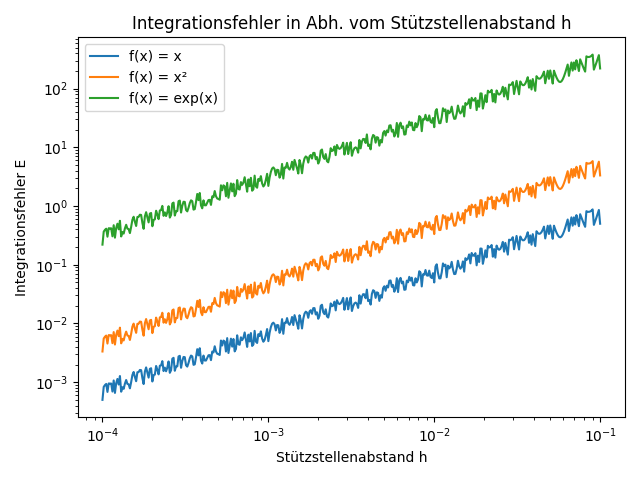
\includegraphics[width=0.5\textwidth]{fig1}
		\caption{Integrationsfehler in Abhängigkeit vom Stützstellenabstand $h$}
	\end{wrapfigure}
	Auf meiner ersten Abbildung sieht man den Integrationsfehler in Abhängigkeit vom Stützstellenabstand $h$. Dieser steigt, wie man sieht polynomiell an (Da wir einen logarithmischen Plot haben, sehen wir dies als lineare Funktion). Der Fehler bei $f(x) = e^x$ ist besonders stark, das liegt daran, dass ich die Fläche unter der Kurve mit Rechtecken approximiere. Je stärker also der Anstieg eine Funktion ist, desto schlechte lässt sie sich durch diese Vereinfachung abschätzen. Das gilt für $f(x) = x^2$ natürlich auch mehr als für $f(x) = x$, wodurch diese ganz klar abgetrennten Fehler entstehen. Die lineare Funktion hat noch den Vorteil, dass jedes Rechteck die Fläche unter der Kurve in seinem Intervall perfekt abschätzt, da der Teil der zu viel, ist auf der anderen Seite zu wenig ist und sich die beiden Effekte genau wegkürzen. Der Fehler entsteht durch Randprobleme, wo nicht immer alles abgeschätzt wird. Man sieht, dass der lineare Fehler immer die Größenordnung des Stützstellenabstands hat. 
	
	Die Schwankungen kommen so zustande, dass bestimmte $h$s das Intervall $[a, b]$ besser teilt (am besten $h|(b-a)$). Wenn wir nämlich ein $h$ nehmen, sodass $\lnot\exists k \in  \N: k \cdot h = b - a$, bleibt am Rand etwas Platz, welcher nicht von Rechtecken approximiert wird. Damit wird, egal von welcher Funktion die Fläche unter der Kurve berechnet wird, dort ein gewisser Fehler gemacht. Desshalb sehen die kleinen Schwankungen bei allen 3 Kurven gleich aus.
	
	\begin{wrapfigure}[20]{r}{0.5\textwidth}
		\centering
		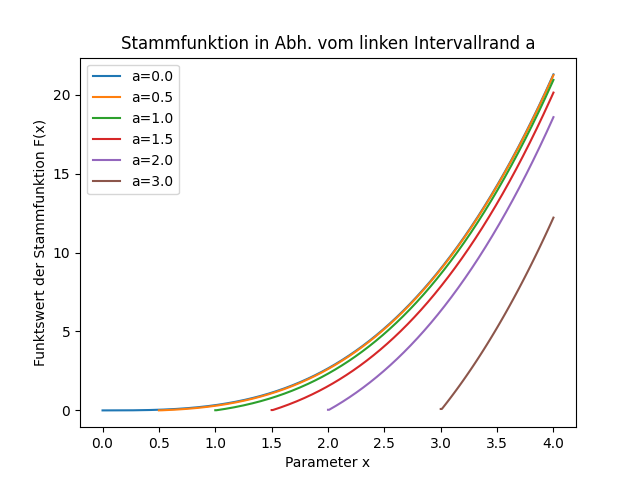
\includegraphics[width=0.5\textwidth]{fig2}
		\caption{Stammfunktion von $f(x) = x^2$ in Abhängigkeit vom linken Intervallrand $a$}
	\end{wrapfigure}

	Auf Abbildung 2 sieht man die numerisch bestimmte Stammfunktion von $f(x) = x^2$ in Abhängigkeit des linken Intervallrands. Natürlich fangen alle Stammfunktionen erst an den jeweiligen Stellen ($x=a$) im Plot an. Außerdem sieht man, dass alle Stammfunktionen überall den selben Anstieg haben, nur sind sie entlang der y-Achse verschoben. Dies ist jedoch kein Problem, da eine in y-Richtung verschobene Stammfunktion immer noch eine Stammfunktion ist. Nun bleibt die Frage, woher kommt das? Da die Stammfunktion $F_a$ mit linken Integrationsrand $a$ durch eine kommulierte Summe der Funktionswerte $f(x)$ ab $a$ berechnet wird, gilt immer $F(a) \approx 0$. Damit gilt für $f(x) = x^2$:
	
	$$F_a(x) = \frac{1}{3}x^3 + c.\qquad F_a(a) = \frac{1}{3}a^3 + c \stackrel{!}{=} 0$$
	$$\Rightarrow\quad F_a(x) = \frac{1}{3}(x^3 - a^3)$$
	
	Und dies wird auch in dem Plot widergespiegelt.

\end{document}
